\documentclass[a4paper, 10pt]{article}

% Typography & Font Handling
%\usepackage[utf8]{inputenc}
\usepackage[T1]{fontenc}
\usepackage{lmodern}
\usepackage{microtype}
\usepackage{fontspec}
\usepackage{sectsty}
\usepackage{fixltx2e}
\usepackage{titlesec}

% Fonts
%\usepackage{garamondlibre}
\setmainfont{Garamond Libre}  % Serif
\setsansfont{TeX Gyre Heros}    % Sans
\setmonofont{TeX Gyre Cursor}  % Mono

% Mathematics
\usepackage{amsmath}
\usepackage{amssymb}
\usepackage{mathtools}

% Numbers
\usepackage{siunitx}
\sisetup{
    detect-all,   % detects the surrounding font
    detect-family,
    detect-shape,
    detect-weight
}

% Lists
\usepackage{enumitem}

% Tables
\usepackage{booktabs}
\usepackage{array}
\usepackage{tabularx}
\newcolumntype{Y}{>{\raggedright\arraybackslash}X}

% Graphics
\usepackage{graphicx}
\usepackage{float}

% Figures
\usepackage{subcaption}
\usepackage{wrapfig}

% Circuits
\usepackage{circuitikz}

% Code Listings
\usepackage{listings}

% Layout & Page Formatting
\usepackage{geometry}
\usepackage{fancyhdr}
%\usepackage{indentfirst}
\usepackage{parskip}
% References
\usepackage{hyperref}
\usepackage{cleveref}

%\usepackage{lipsum}

%============================================
\geometry{
headheight=25pt,
top=1in,
bottom=1in,
left=0.5in,
right=0.5in
}
\title{ELEC ENG 2411 Ex: 3\vspace{5em}
}
\author{
	{\Large Prepared by:}\\
	Lucas Rufkahr\vspace{5em}\\
	%{\Large In Collaboration with:}\\
	%Aiden Burns\vspace{5em}\\
	{\Large Submitted to:}\\
	Sokrat Aldarmini\vspace{5em}\\
	{\Large Submitted on:}\\
	\today
}
\date{}

\titleformat*{\section}{\Large\bfseries\sffamily}
\renewcommand{\thesection}{\arabic{section}}
\titleformat*{\subsection}{\large\bfseries\sffamily}
\renewcommand{\thesubsection}{\thesection.\Alph{subsection}}
\titleformat*{\subsubsection}{\itshape\sffamily}
\renewcommand{\thesubsubsection}{\thesubsection.\roman{subsubsection}}

\begin{document}
\setcounter{secnumdepth}{4}
\pagestyle{fancy}
\fancyhead[L]{Lucas Rufkahr}%, Aiden Burns}
\fancyhead[C]{Experiment 2}
\fancyhead[R]{EE2411 --- Section 305\\\today}
\maketitle
\thispagestyle{empty}
%========================
\pagebreak
\section*{Part 1 Step 1}
We first create a vector T that runs from 0 to 10. We then execute a conditional statement \texttt{T==5}. This creates a variable \texttt{ans} with a type of vector. It has the same size of T except T is a double vector whereas ans is a logical vector. It is filled with zeroes except the position of 5 in T is equal to 1 in ans.
\section*{Part 1 Step 2}
We create a new function called \texttt{unitStep()} in a new file named \texttt{unitStep.m}. This function takes a vector as an input and outputs another vector with the same dimensions. Where the values of t are greater than zero, we set the y vector to one and everywhere else to zero. This resulting output is a unit step function.
\section*{Part 1 Step 3}
We first create a variable \texttt{t} using the \texttt{linspace()} function from -2 to 4 with 1000 points. We do this because we want to plot $x(t) = e^{-2t}(u(t) - u(t-1))$ and the 1000 points in between our interval will give us a smooth plot. We then create a variable \texttt{x =  exp(-2 * t) .* (unitStep(t) - unitStep(t - 1));} We then use the functions \texttt{plot(t,x)}, \texttt{title('')}, \texttt{xlabel('')}, and \texttt{ylabel('')} to create the plot, set the title, and label the x and y axes. \texttt{exportgraphics()} was then used to render the figure to a PNG file. In figure \ref{fig:part1_step3} we can see the exponential function is zero for every t less than zero and greater than 1. The only region where the exponential behavior shows is from zero to one. Clearly we can see that the unit step function that was defined in Part 1 Step 2 is behaving normally.
\begin{figure}[H]
        \centering
        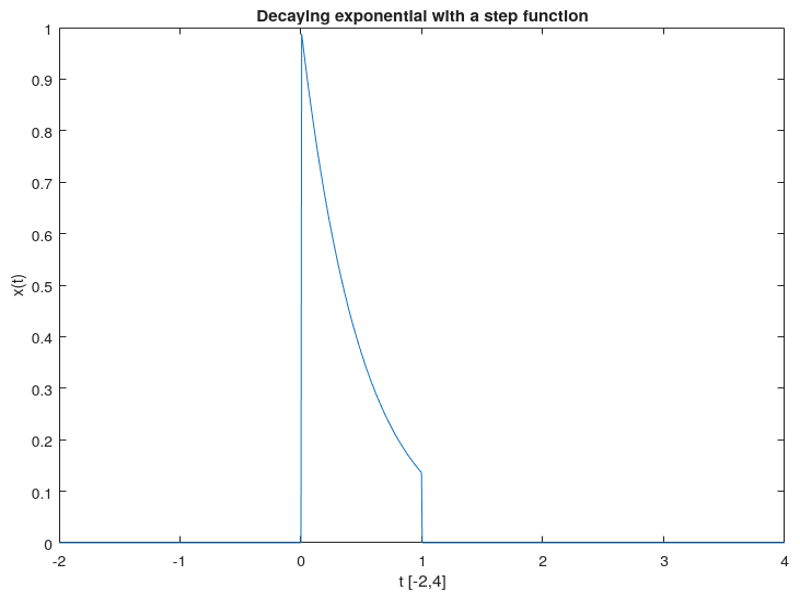
\includegraphics[scale=1]{./assets/part1/part1_step3.png}
	\caption{A decaying exponential multiplied by a step function from 0 to 1.}
	\label{fig:part1_step3}
\end{figure}
\section*{Part 1 Step 4}
We now want to plot $x(t - 1.5)$. To do this, we need to define a new variable \texttt{x\_shift} which is essential a copy of our original x except where t was, we replace with \texttt{(t - 1.5)}. We also want to plot this on top of our previous plot. To do this, we use the \texttt{hold on} statement and then we invoke the \texttt{plot(t,x\_shift)} function. We now want to also plot $x(2t)$, and $x(-t)$ on top of the same figure as well which can be done using the same logic as before. To add a legend to our figure, we invoke the \texttt{legend()} function. Labels are applied in the order the \texttt{plot()} function was called so we create the exponential first, shifted, compressed, and then reversed. The plot for this figure is shown in figure \ref{fig:part1_step4}.

We can also calculate the energy of our functions. We use function \texttt{trapz()} which approximates the integral of a vector over an interval. We want to approximate the energy of $x(t)$, $x(t - 1.5)$, and $x(2t)$. To check the output of the function, we can also calculate this by hand. The formula for the trapezoidal method is equation \ref{eq:trapezoidal_method} where $\Delta x = \frac{b - a}{n}$ and $x_{i} = a + i \Delta x$.
\begin{equation}
	\int_{a}^{b}{f(x)}{dx} \approx \frac{\Delta x}{2}\bigl(f(x_0) + 2f(x_1) + 2f(x_2) + ... + 2f(x_{n-1}) + f(x_n)\bigr)
	\label{eq:trapezoidal_method}
\end{equation}
To find the energy of a function, we need to take the absolute value of the function and square it. We also use the bounds of $(-\infty , \infty)$. Our equation becomes equation \ref{eq:energy_trapezoidal_method}.
\begin{equation}
	E = \int_{- \infty}^{\infty}{\lvert f(x) \rvert ^2}{dx} \approx \frac{\Delta x}{2}\bigl(\lvert f(x_0) \rvert ^2 + 2\lvert f(x_1) \rvert ^2 + 2 \lvert f(x_2) \rvert ^2 + ... + 2 \lvert f(x_{n-1}) \rvert^2 + \lvert f(x_n) \rvert ^2 \bigr)
	\label{eq:energy_trapezoidal_method}
\end{equation}
We begin by equating our bounds to $a$ and $b$ as it is where $x(\alpha x + \tau) > 0$ since everywhere else it is zero. For $n$, we will use 4 subintervals to preserve time. The energy equations are:
\begin{equation}
	E_{x(t)} = \int_{0}^{1}{\lvert x(t) \rvert ^2}{dx} \approx \frac{1}{8}\bigl(1 + 0.368 + 0.271 + 0.100 + 0.018 \bigr) = 0.265
\end{equation}
\begin{equation}
	E_{x(t - 1.5)} = E_{x(t)}
\end{equation}
\begin{equation}
	E = \int_{0}^{0.5}{\lvert x(2t) \rvert ^2}{dx} \approx \frac{\Delta x}{2}\bigl(1 + 0.736 + 0.271 + 0.100 + 0.183 \bigr) = 0.133
\end{equation}
Now that we've manually calculated the energies using a small resolution, we can see that our results are similar to but not exactly to the MATLAB calculated. Results are summarized in table \ref{tab:trapezoidal_energy}.
\begin{table}[H]
	\centering
	\begin{tabularx}{0.7\linewidth}{YYYY}
		Function & Energy (MATLAB) & Energy (Manual; n=4) \\
		$x(t)$ & 0.24243 & 0.265 \\
		$x(t - 1.5)$ & 0.24695 & 0.265 \\
		$x(2t)$ & 0.11976 & 0.133
	\end{tabularx}
	\caption{Approximated integral using \texttt{trapz} compared to hand calculation with n = 4}
	\label{tab:trapezoidal_energy}
\end{table}
To demonstrate why it is important to using a vector with a sufficiently large step size or resolution, we recreate our $x(t)$ using a time vector with a step size of one. The resulting energy when using the trapz function is near zero and is sufficiently smaller than our calculation using a time vector created with linspace and a resolution of 1000. Without a sufficiently large step size, the approximation is insufficiently accurate because a proper shape cannot be formed within the curve.

Now lets focus on the curve $x(-t)$. If we were to consider the output of a physical system, we need to make the assumption that the system is a causal system. The nature of a causal system is that for all $t < 0$, the output of the system must be zero. Now under the assumption that we are considering the output of a causal system, it then would not make sense if $x(-t)$ was the output because it does not agree with our criterion stated before.
\begin{figure}[H]
        \centering
        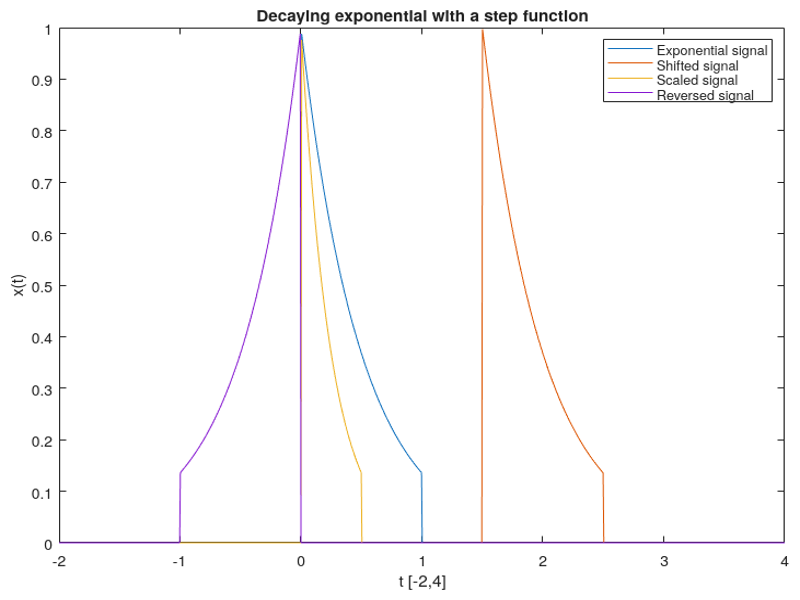
\includegraphics[scale=1]{./assets/part1/part1_step4.png}
	\caption{A plot of four curves, $x(t)$, $x(t - 1.5)$, $x(2t)$, and $x(-t)$.}
        \label{fig:part1_step4}
\end{figure}
\section*{Part 1 Step 5}
This step concerns the \texttt{subplot()} function. We want each function: $x(t)$, $x(t - 1.5)$, $x(2t)$, $x(-t)$; to be plot on a new figure with each function on their own separete axis. We begin by creating a new figure with \texttt{figure()} and then calling \texttt{subplot(m, n, p)}. Since we have four plots, we want $m = n = 2$. We first call \texttt{subplot()} with $p = 1$ can then we call \texttt{plot} for our $x(t)$. We then call our title and label functions to add them. Next with $p = 2$ we call \texttt{subplot()} again and then repeat the \texttt{plot()} function, title, and labels for $x(t - 1.5)$. Then we repeat this for the remaining functions with $p = 3$ and $p = 4$. The resulting figure is shown in figure \ref{fig:part1_step5}.

We can also adjust the axis limits and enable the grid after we plot our functions just by calling \texttt{subplot()} to select the subplot we want to adjust. We use \texttt{xlim([i n])} to adjust the interval of the x-axis, and \texttt{grid on} to enable to grid. The figure with these extra modifications is shown in figure \ref{fig:part1_step5_grid}.
\begin{figure}[H]
	\centering
	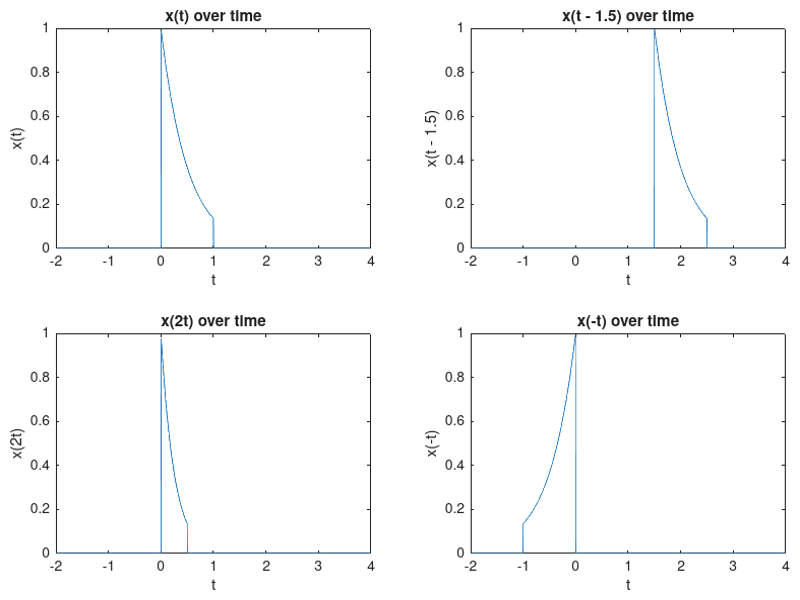
\includegraphics[scale=1]{./assets/part1/part1_step5.png}
	\caption{A figure containing four plots: $x(t)$, $x(t - 1.5)$, $x(2t)$, and $x(-t)$.}
	\label{fig:part1_step5}
\end{figure}
\begin{figure}[H]
	\centering
	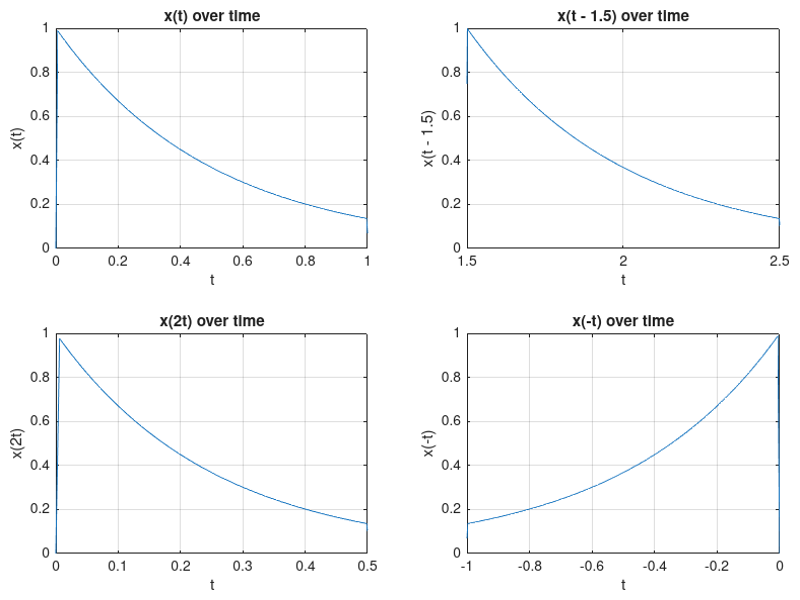
\includegraphics[scale=1]{./assets/part1/part1_step5_grid.png}
	\caption{Modified figure \ref{fig:part1_step5} with each with a grid and adjusted x-axis interval.}
	\label{fig:part1_step5_grid}
\end{figure}
\section*{Part 1 Step 6}
In this step we will demonstrate how MATLAB can be used to interpret systems information as audio data. For this, we will consider the function $y(t) = sin\bigl(2\pi(f_0t + 0.5\beta t^2)\bigr)$ where $\beta = (f_1 - f_0)/T$, $f_0$ is the starting frequency, $f_1$ is the end frequency, and $T$ is the duration. First we create a variable \texttt{freq\_samp} equal to 441kHz. We then create a variable \texttt{T\_samp} or the sampling period equal to one over the sampling frequency. Next we create our time domain vector which is a vector from zero to four with a step size equal to that of our sampling period. We will start with a frequency of 20Hz and work up to a frequency of 200Hz. We then create a variable \texttt{beta} and then define our function variable \texttt{y = sin(2 * pi * (freq\_0 * t + 0.5 * beta * t.\^{}2));}. Next we create a new figure and plot our function y. We set the x-axis interval from 0 to 2 and our y-axis interval from -1.5 to 1.5. The resulting plot is shown in figure \ref{fig:part1_step6}. We can see that the frequency increases as time increases. Using the \texttt{soundsc} function, we can play the sound and we hear that it is a sine wave increasing in frequency. To play this in reverse, we can use the \texttt{fliplr} function. If we play this reversed data, we can hear that it is a sine wave decreasing in frequency. We can also multiply t by two and divide t by two to create audio data that increases quicker and slower in frequency respectively. We can also create audio data that decreases in frequency and then increases by using concatenation. To do this, we define a new variable \texttt{fall\_rise = [y\_reversed, y]}. Playing this data, we can see that the frequency starts high, decreases, then rises again.
\begin{figure}[H]
	\centering
	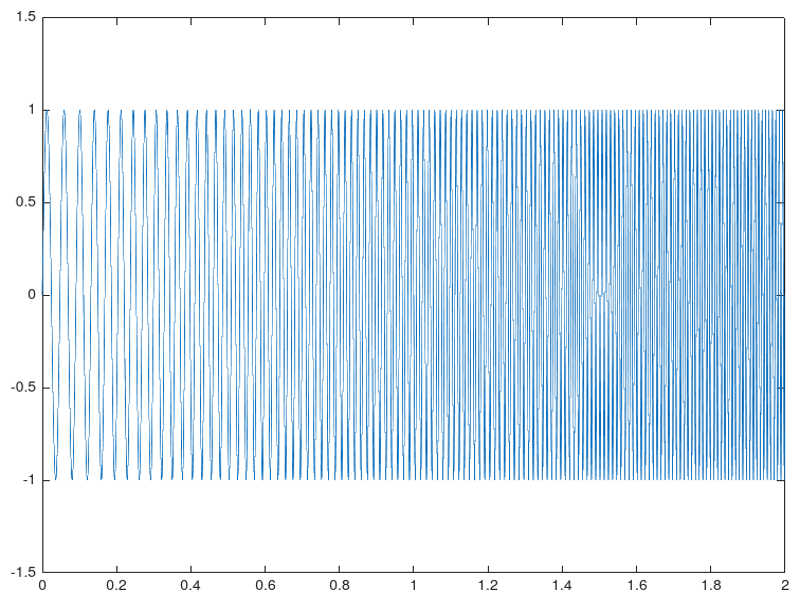
\includegraphics[scale=1]{./assets/part1/part1_step6.png}
	\caption{Audio signal starting at 20Hz and increasing linearly to 200Hz as time increases.}
	\label{fig:part1_step6}
\end{figure}
\section*{Part 2 Step 1}
In part 2, we will work with three-dimensional data objects. We want to create a surface which we will do using the \texttt{surf()} function. First we define x and y vectors from -4 to 4 with a step size of 0.01. We create matrices which will serve as the x and y planes. We do this using the statement \texttt{[X,Y] = meshgrid(x,y)}. Net we will create another matrix which will serve as the Z element in our three dimensions. We define \texttt{Z = 2 * cos(X) - sin(Y.\^{}2)}. Now we use the \texttt{surf()} function with paremeter \texttt{EdgeColor='none'}. We then add x and y labels to our figure. The resulting figure is shown in figure \ref{fig:part2_step1}.
\begin{figure}[H]
	\centering
	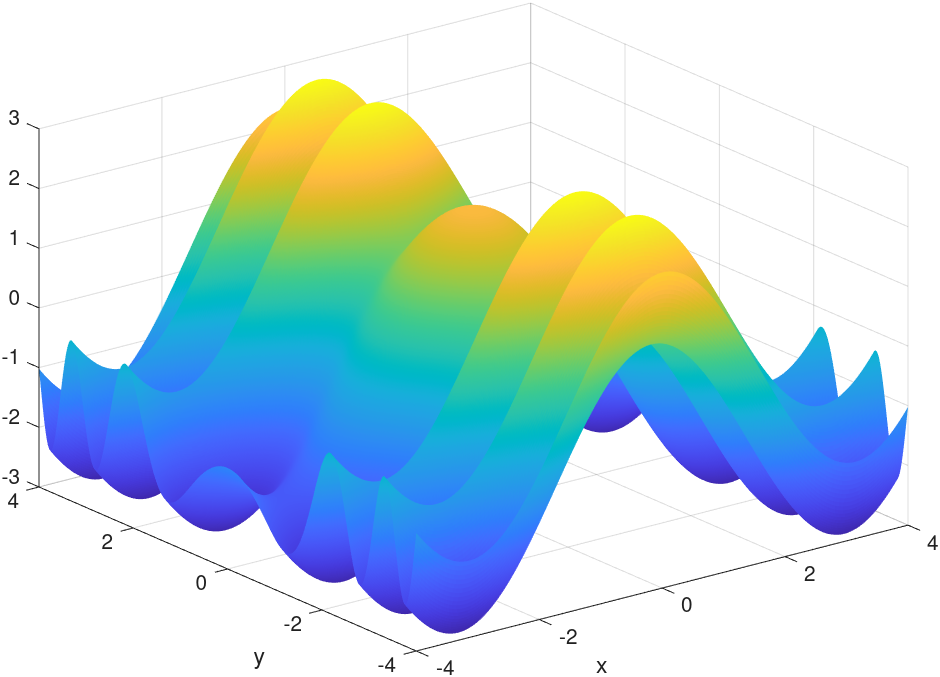
\includegraphics[scale=1]{./assets/part2/part2_step1.png}
	\caption{A three dimensional surface plot.}
	\label{fig:part2_step1}
\end{figure}
\section*{Part 2 Step 2}
Now we will work with image data. In MATLAB, images are nothing but three dimensional objects. We will use stock MATLAB images and manipulate their data to give different results. First we load image data by defining a new variable \texttt{imData = imread('office\_6.jpg')}. The function \texttt{imread()} will read the JPEG data from office\_6.jpg and turn it into a three dimensional object that we can manipulate. We can show the figure using the \texttt{imshow()} function. The \texttt{imData} variable that was created contains pixel data in order of rows and columns. It also contains pages which correspond to individual color channels. We can show a red version of office\_6.jpg by all color channels except red. We first create a new variable \texttt{imData1} as a copy of our original image data. Then we execute statements that set page two and three to zero. The resulting image is shown in figure \ref{fig:part2_step2_red}. We can also remove color channel data such that the resulting image is yellow. To do this, we only remove the third color channel so that only red and blue remain. This is done by setting page three to zero. The image is shown in figure \ref{fig:part2_step2_yellow}.
\begin{figure}[H]
	\centering
	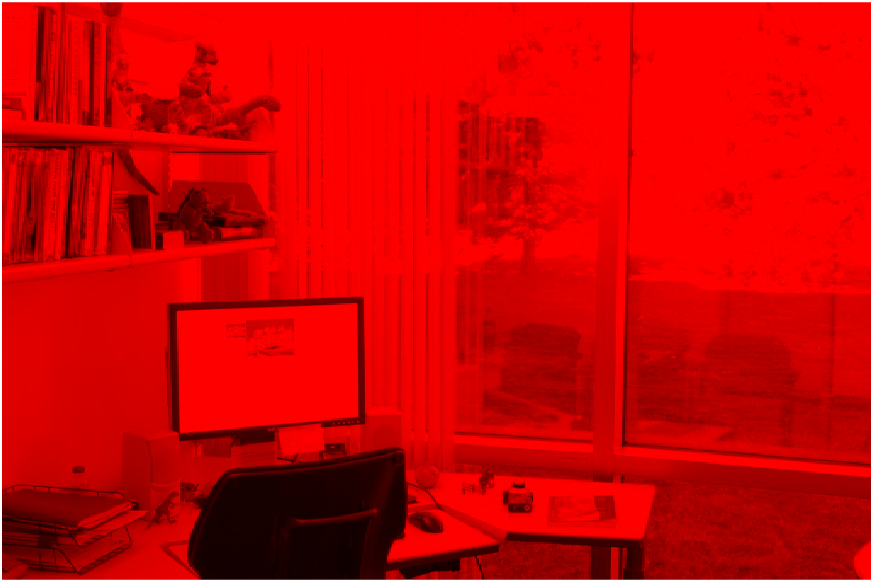
\includegraphics[scale=1]{./assets/part2/part2_step2_red.png}
	\caption{office\_6.jpg with only red color channel data.}
	\label{fig:part2_step2_red}
\end{figure}
\begin{figure}[H]
	\centering
	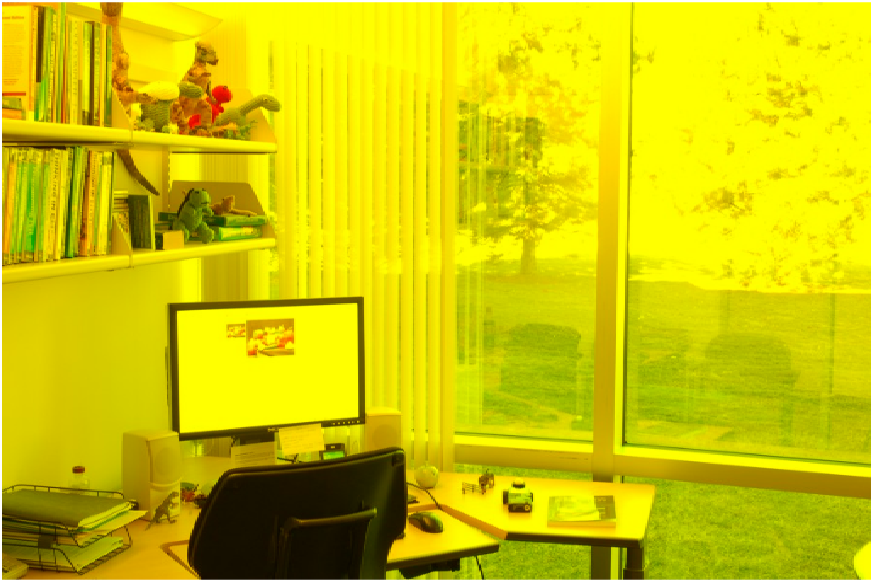
\includegraphics[scale=1]{./assets/part2/part2_step2_yellow.png}
	\caption{office\_6.jpg with red and blue color channel data.}
	\label{fig:part2_step2_yellow}
\end{figure}
We can also manipulate the size of the image. This is done by only selecting rows and columns that one whishes to show. We will demonstrate this by showing only the bottom half and removing the end quarter of the image. To do this, we create a new variable \texttt{sliceImData = imread('office\_6.jpg')}. Next we set our variable equal to only the data we require. Using the colon operator, we can select ranges of data.We do this by executing the statement \texttt{sliceImData = sliceImData(end*0.5:end, 1:end*0.75,:)}. The first argument selects the row at the halfway point up to the last row. The second argument selects the first column up to 3/4 of all the columns. The last argument selects all the pages because want to keep the color data as it originally is. The resulting image is shown in figure \ref{fig:part2_step2_crop}.
\begin{figure}[H]
	\centering
	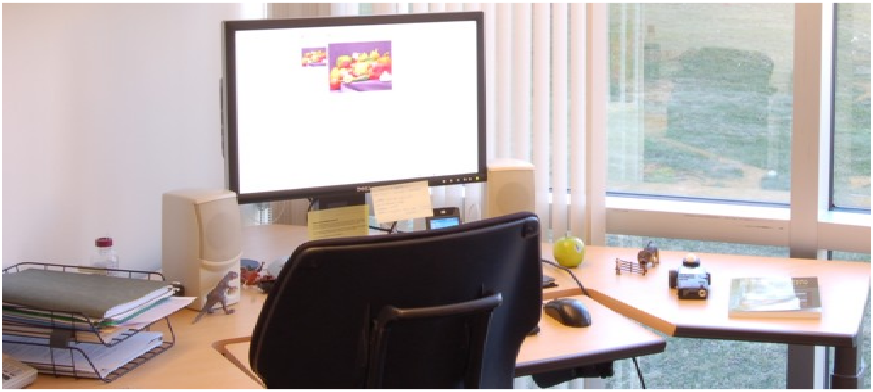
\includegraphics[scale=1]{./assets/part2/part2_step2_crop.png}
	\caption{office\_6.jpg with selectively chosen rows and columns.}
	\label{fig:part2_step2_crop}
\end{figure}
We can also manipulate color data so that only brightness data is shown. We can do this by using the function \texttt{rgb2gray()}. We create a new variable \texttt{imDataG} equal to the grayscale function with image data as its only argument. The resulting image is shown in figure \ref{fig:part2_step2_gray}. We can also perform image normalization using equation \ref{eq:image_normalization}.
\begin{figure}[H]
	\centering
	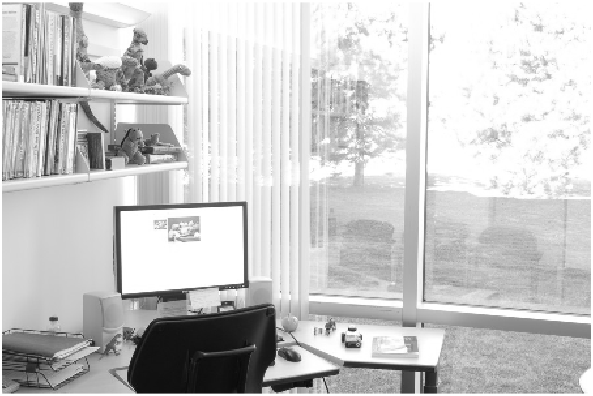
\includegraphics[scale=1]{./assets/part2/part2_step2_gray.png}
	\caption{office\_6.jpg converted to grayscale.}
	\label{fig:part2_step2_gray}
\end{figure}
\begin{equation}
	\textrm{newData} = (\textrm{oldData} - \textrm{oldMin}) \times \frac{\textrm{newMax} - \textrm{newMin}}{\textrm{oldMax} - \textrm{oldMin}} + \textrm{newMin}
	\label{eq:image_normalization}
\end{equation}
We first define \texttt{newMin = 2 * min(imDataGSF, [], 'all')} and \texttt{newMax = 0.5 * max(imDataGSF, [], 'all')} to create minimums that are twice as bright as the old minimums and maximums that are half as bright as the old maximums. The resulting image is shown in figure \ref{fig:part2_step2_brightness}. A table showing minimum and maximum intensity before and after is shown in table \ref{tab:part2_step2_brightness}.
\begin{figure}[H]
	\centering
	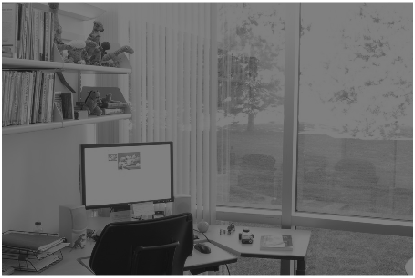
\includegraphics[scale=1]{./assets/part2/part2_step2_brightness.png}
	\caption{office\_6.jpg with image normalization applied.}
	\label{fig:part2_step2_brightness}
\end{figure}
\begin{table}[H]
	\centering
	\begin{tabularx}{0.7\linewidth}{YYY}
		 & Minimum & Maximum \\
		Old & 8 & 255 \\
		New & 16 & 127.5 \\
	\end{tabularx}
	\caption{Minimum and maximum brightness data before and after normalization.}
	\label{tab:part2_step2_brightness}
\end{table}
\end{document}
